\documentclass[english,a4paper,twoside]{article}
\usepackage{autiwa}
\usepackage{aas_macros}

\title{Nautilus Documentation}
\author{Christophe Cossou}

\newcommand{\raccourci}[1]{{\bfseries #1}}
\newcommand{\molecule}[1]{\ensuremath{\mathrm{#1}}}

\makeindex
\begin{document}

\begin{titlepage}
\begin{center}
~
\vfill
% Upper part of the page
\begin{figure}[t]
\centering
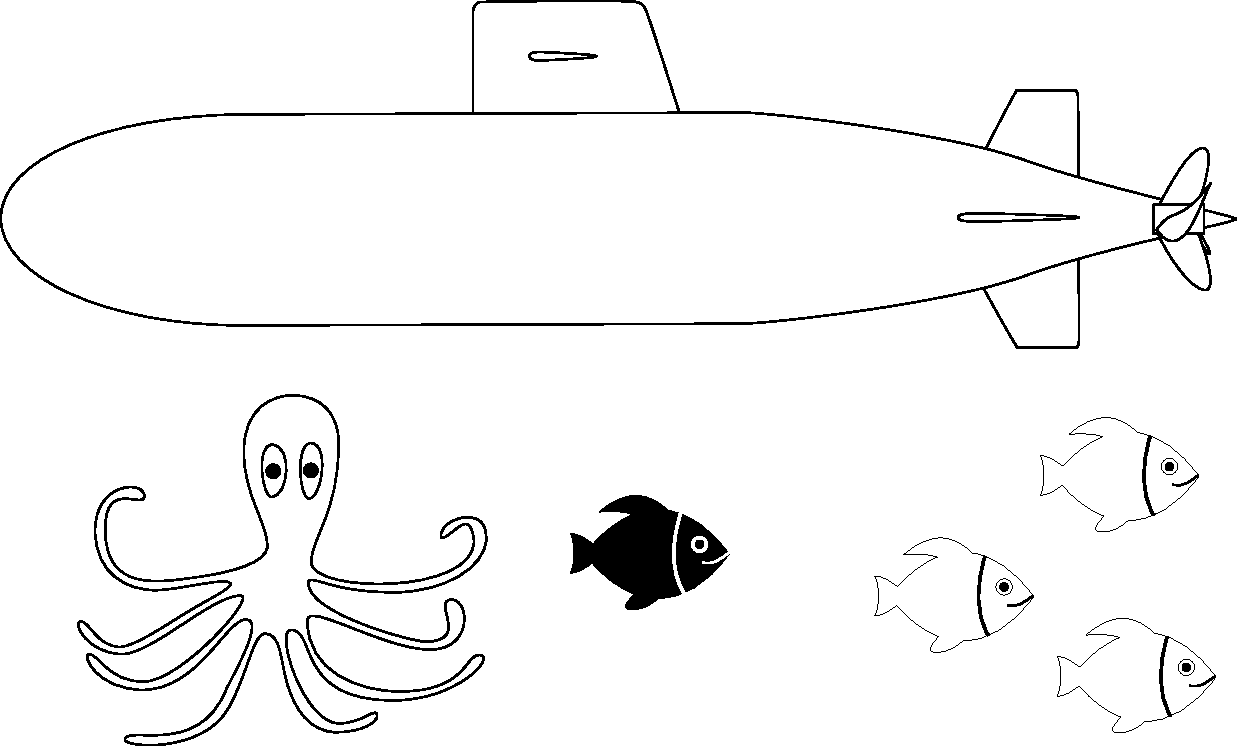
\includegraphics[width=0.5\textwidth]{figures/nautilus_logo.pdf}%chemin absolu de l'image pour que l'on puisse appeler ce fichier depuis plusieurs dossiers différents.
\end{figure}

% Title
\HRule \\[0.4cm]
{ \huge \bfseries \makeatletter\@title\makeatother}\\[0.4cm]

\HRule \\[0.75cm]
{\large \today}\\[0.75cm]
\makeatletter
\@author
\makeatother
\vfill
\vfill
~
% Bottom of the page


\end{center}
\end{titlepage}

\cleardoublepage

\tableofcontents

\cleardoublepage

\section{Starting with Nautilus}
From all the python script that come with the code, you can see all parameters and sometimes a few examples by typing:
\begin{verbatim}
script_name.py help
\end{verbatim}

\begin{attention}
Beware, \textbf{nautilus} is generally the default file browser in GNU/Linux Gnome environment. Thus, by typing \textbf{nautilus} in a terminal, you will not launch the simulation program, but rather the X server and everything that comes with it (if you're in a remote SSH connection).
\end{attention}

For all input files, the comment character is " !" and can be either at the beginning of a line, or anywhere else. Meaningful character must be comprised inside the 80th first characters of a given line.

\gras[input file!parameters.in]{parameters.in} is the main parameter file, and is rewritten by the code itself each and every time you run the code. 

\subsection{Generic informations about parameter files}\label{sec:files_generic_info}
By default, the character "!" comment everything after it. If a line start with it, the line will be completely ignored.

\subsection{Getting the Git repository}
First, you need to get the Git repository from \gras{Googlecode} before actually using the code. 

I assume you only want to use it, without ever putting on the distant repository anything. This way, you don't even need to have an account and a password. 

In the parent directory where you want to put a \textbf{nautilus} folder containing the Git repository, type:
\begin{verbatim}
git clone https://code.google.com/p/nautilus/
\end{verbatim}

\subsection{Compilation}
The script \gras{Makefile.py} allow you to compile the code. The default compiler is \gras{gfortran}. 

If you want to just run the code, type:
\begin{verbatim}
Makefile.py
\end{verbatim}

\begin{remarque}
Errors in log files associated with the module incriminated. Warnings are stored in a generic file \gras{compilation.log}.
\end{remarque}

\begin{attention}
By default, all warnings issued by \gras{ODEPACK} routines are masked (to increase readability, since nobody can modify this thing from scratch). An option can force their display.
\end{attention}

If you want to compile the binary \gras[binary!nautilus\_outputs]{nautilus\_outputs} that generate ASCII from the binary outputs:
\begin{verbatim}
Makefile.py output
\end{verbatim}

If you want to compile the binary \gras[binary!nautilus\_rates]{nautilus\_rates} that generate analysis of reaction rates:
\begin{verbatim}
Makefile.py rates
\end{verbatim}

If you want to compare versions of the code \ref{sec:compare_simulation}, type:
\begin{verbatim}
Makefile.py test
\end{verbatim}
The option \textbf{test} use compilation options that allow comparison of the code between different versions. 

\subsection{Usefull tools}
\subsubsection{Git Prompt}
You can display in your terminal useful information about a Git repository by modifying your bash profile (assuming you terminal uses Bash, which is also always the case).

Add in your \gras{.bashrc} or \gras{.bash\_profile}:
\begin{verbatim}
#########################################
# personnalisation du prompt avec la branche du projet git
#########################################

git_branch_name_prompt() {
    # Only do this if the current directory is a git repository
    if git status 2>/dev/null 1>/dev/null ; then
        # We keep only the first line, then the last word is our branch
        git_status_output=$(git status 2> /dev/null|head -1) || return

        branch_name() {
        # We get the last word with grep
            echo "$git_status_output"|grep -oE '[^ ]+$' 
        }
    
    
        echo "($(branch_name))"
    fi
}

git_branch_colour_prompt() {
    # Only do this if the current directory is a git repository
    if git status 2>/dev/null 1>/dev/null ; then
        git_status_output=$(git status 2> /dev/null) || return

        find_pattern_in_status() {
            local pattern="$1"
            [[ "$git_status_output" =~ ${pattern} ]]
        }

        is_clean() {
            local clean_fr='(rien à valider, la copie de travail est propre)'
            local clean_en='(working directory clean)'
            find_pattern_in_status "($clean_fr|$clean_en)"
        }

        is_local_changes() {
            local added_fr='Modifications qui seront validées :'
            local not_added_fr='Modifications qui ne seront pas validées :'
            local added_en='# Changes to be committed'
            local not_added_en='# Changes not staged for commit'
            find_pattern_in_status "($added_fr|$not_added_fr|$added_en|$not_added_en)"
        }

        is_untracked() {
            local untracked_fr='Fichiers non suivis:'
            local untracked_en='# Untracked files'
            find_pattern_in_status "($untracked_fr|$untracked_en)"
        }

        # local bold="\033[1m"
        local no_colour="\033[0m"
        local red="\033[31m"
        local green="\033[32m"
        local yellow="\033[33m"
        local branch_colour=""

        if is_untracked
        then
            branch_colour=$red
        elif is_local_changes
        then
            branch_colour=$yellow
        elif is_clean
        then
            branch_colour=$green
        fi

        echo -e "$branch_colour"
    fi
}

PS1="\h.\u:\[\033[35m\]\W\[\033[0m\]\[\$(git_branch_colour_prompt)\]\$
(git_branch_name_prompt)\[\033[0m\]\$ "
\end{verbatim}

\subsection{Input files}
An example simulation, containing all necessary input files is provided in the subfolder \textbf{example\_simulation}.

\begin{attention}
All input files have the same \textbf{*.in} extension.
\end{attention}

The main parameter file is \gras[input file!parameters.in]{parameters.in} (see \refsec{sec:parameters_in}).

\gras[input file!abundances.in]{abundances.in} give initial abundances for a set of species (not necessarily all of them). Default minimum values are applied to the species not present in this file (this value is set by the parameter \verb|minimum_initial_abundance| in \gras[input file!parameters.in]{parameters.in} (see \refsec{sec:parameters_in}).

\gras[input file!element.in]{element.in} name and mass in Atomic mass unit of all prime elements existing in the simulation (base elements used to construct molecules).

There are 2 parameter files listing all reactions in a given phase (gas or grain): 
\begin{itemize}
\item \gras[input file!gas\_reactions.in]{gas\_reactions.in}
\item \gras[input file!grain\_reactions.in]{grain\_reactions.in}
\end{itemize}
and 2 parameter files for species present in a given phase (gas or grain) reactions:
\begin{itemize}
\item \gras[input file!gas\_species.in]{gas\_species.in}
\item \gras[input file!grain\_species.in]{grain\_species.in}
\end{itemize}

\begin{remarque}
Species in \gras[input file!gas\_species.in]{gas\_species.in}, \gras[input file!grain\_species.in]{grain\_species.in} are not necessarily species from one phase. These are species \emph{involved} in a given phase reaction. But adsorption or desorption transform grain species into gas species, and vice versa. 
\end{remarque}

\gras[input file!activation\_energies.in]{activation\_energies.in} provide activation energies for some endothermic reactions. 

\gras[input file!surface\_parameters.in]{surface\_parameters.in} provide information about various energies and parameters for diffusion and movements on the grain surface.

\section{Test of the code}
\subsection{Automatic test before computation}
In \gras[input file!parameters.in]{parameters.in}: 
\begin{verbatim}
preliminary_test = 1
\end{verbatim}\index{parameter!preliminary\_test}

When set to 1, the parameter \gras[parameter!preliminary\_test]{preliminary\_test} will allow you to test thoroughly the chemical network. 

\begin{remarque}
This parameter should be set to 0 only in the case of intensive campaign of simulations using the very same network, to avoid wasting computation time doing the sames tests. But in any other cases, I advice you to leave it activated, because it only take around 1 second at the beginning of the simulation.
\end{remarque}

The tests currently made are:
\begin{itemize}
\item Check that grain species (read from \gras[input file!grain\_species.in]{grain\_species.in}) are indeed grain species
\item Check that all species gave production AND destruction reactions (error if none, warning if only one)
\item Check that each reaction is equilibrated in prime element and in electric charge
\item Display a warning for each reaction having alpha=0 (first parameter for reaction rate formula
\item Check that $T_\text{min} < T_\text{max}$ for each reaction
\item For reaction with the same ID:
\begin{itemize}
\item Check that they have the same reactants and products
\item Check that temperature ranges do not overlap.
\end{itemize}
\item Check that each gas neutral species have a grain equivalent (excluding \textbf{GRAIN0} and \textbf{XH}).
\item Check that each gas neutral species has an adsorption reaction (ITYPE=99) (excluding \textbf{GRAIN0} and \textbf{XH}).
\item Check that each grain species has at least one reaction of each of the following types: 15, 16, 66, 67 (desorption reactions).
\item Check that all index ranges associated with a reaction type join themselves to cover all the index range of all reactions.
\end{itemize}

\section{Parameter file : parameters.in}\label{sec:parameters_in}\index{input file!parameters.in}
For generic informations, see \refsec{sec:files_generic_info}.

\gras[input file!parameters.in]{parameters.in} has the particularity to be re-written each time you launch a Nautilus simulation. This ensure several things :
\begin{itemize}
\item Parameters can be input in random ways, the code will sort them by categories
\item New parameters, with default values will be added, to ensure retro-compatibility.
\end{itemize}

\subsection{Simulation parameters}
\begin{verbatim}
start_time =  1.000E+00
\end{verbatim}\index{parameter!start\_time}
In years, the first output time of the simulation (all simulation starts from $T=0$).

\begin{verbatim}
stop_time =  1.000E+01
\end{verbatim}\index{parameter!stop\_time}
End of the simulation in years (and also the last output time)

\begin{verbatim}
nb_outputs =    3
\end{verbatim}\index{parameter!nb\_outputs}
Total number of outputs (including \verb|start_time| and \verb|stop_time|. This number will be used when \gras[parameter!output\_type]{output\_type} is \textbf{log} or \textbf{linear}.

\begin{verbatim}
output_type = log
\end{verbatim}\index{parameter!output\_type}
Define the type of output you want. Possible values are \textbf{linear}, \textbf{log}, and \textbf{table}. 
\begin{itemize}
\item \textbf{linear} : The spacing between the different output times will be linear
\item \textbf{log} : The different output times will be log-spaced.
\item \textbf{table} : The different output times are read from the file \gras[input file!structure\_evolution.dat]{structure\_evolution.dat}. The parameter \gras[parameter!nb\_outputs]{nb\_outputs} is then completely ignored.
\end{itemize}

\begin{verbatim}
relative_tolerance =  1.000E-04
\end{verbatim}\index{parameter!relative\_tolerance}
Relative tolerance of the solver

\begin{verbatim}
minimum_initial_abundance =  1.000E-40
\end{verbatim}\index{parameter!minimum\_initial\_abundance}
default minimum initial fraction abundance applied to species whose abundance is not specified in \gras[input file!abundances.in]{abundances.in}.

\subsection{Time evolution of the physical structure}\index{parameter!is\_structure\_evolution}
\begin{verbatim}
is_structure_evolution = 1
\end{verbatim}\index{parameter!is\_structure\_evolution}

If set, the physical structure we define will evolve with time. This evolution will be read from the file \gras[input file!structure\_evolution.dat]{structure\_evolution.dat} that must exist in the simulation folder. 

This file will have the following format:
\begin{verbatim}
! time    log(Av)    log(n)    log(T)
! (Myr)   (mag)      (cm-3)    (K)
0.000e+00 -1.231e+00 1.813e+00 1.698e+00
2.360e-01 -1.233e+00 1.758e+00 1.712e+00
\end{verbatim}
We define respectively time, visual extinction, gas density and gas temperature. 

Optionally, one can add a 5\th column to define also grain temperature:
\begin{verbatim}
! time    log(Av)    log(n)    log(Tg)     log(Td)
! (Myr)   (mag)      (cm-3)    (K)          (K)
0.000e+00 -1.231e+00 1.813e+00 1.698e+00 1.500e+00
2.360e-01 -1.233e+00 1.758e+00 1.712e+00 1.510e+00
\end{verbatim}
If so, the parameter \gras[parameter!grain\_temperature\_type]{grain\_temperature\_type} must be set to:
\begin{verbatim}
grain_temperature_type = table
\end{verbatim}\index{parameter!grain\_temperature\_table}

\subsection{Grain temperature}
You have four ways of defining grain temperature in the code. The parameter \gras[parameter!grain\_temperature\_type]{grain\_temperature\_type} can have the following values:
\begin{itemize}
\item[\textbf{fixed}] The grain temperature is fixed throughout the simulation, to the value given in \gras[parameter!initial\_dust\_temperature]{initial\_dust\_temperature} ;
\item[\textbf{gas}] The grain temperature is equal to the gas temperature, no matter what.
\item[\textbf{computed}] The grain temperature is calculated following an energy equilibrium with the gas in the structure
\item[\textbf{table}] The grain temperature is then interpolated from the 5\th column of the  \gras[input file!structure\_evolution.dat]{structure\_evolution.dat} file. \gras[parameter!is\_structure\_evolution]{is\_structure\_evolution} must be set to $1$.
\end{itemize}

\subsection{Switches}
To activate (or not) accretion on dust grains and grain surface reactions:
\begin{verbatim}
is_grain_reactions = 1
\end{verbatim}\index{parameter!is\_grain\_reaction}

To activate (or not) the self-shielding of $\molecule{H_2}$ and $\molecule{CO}$, related to visual extinction: 
\begin{verbatim}
is_absorption = 1
\end{verbatim}\index{parameter!is\_absorption}

To activate (or not) grain tunneling diffusion (and choose the type of grain tunneling diffusion: 
\begin{verbatim}
grain_tunneling_diffusion = 0
\end{verbatim}\index{parameter!grain\_tunneling\_diffusion}

Different types are:
\begin{itemize}
\item[0] : Thermal for H, \molecule{H_2}
\item[1] : Quantum tunneling diffusion rate [\unit{s^{-1}}] \citep{1976RvMP...48..513W}
\item[2] : Quantum tunneling diffusion rate [\unit{s^{-1}}] \citep{1992ApJS...82..167H}
\item[3] : Choose fastest
\end{itemize}

To choose whether or not we can modify some rates:
\begin{verbatim}
modify_rate_flag = 1
\end{verbatim}\index{parameter!modify\_rate\_flag}

Different types are:
\begin{itemize}
\item[-1] : H+H only
\item[1] : modify H
\item[2] : modify H,\molecule{H_2}
\item[3] : modify all
\end{itemize}

\subsection{Gas parameters}


\begin{verbatim}
initial_gas_density =  2.000E+04
\end{verbatim}\index{parameter!initial\_gas\_density}
initial gas density in $\unit{particule/cm^{-3}}$

\begin{verbatim}
initial_gas_temperature =  1.000E+01
\end{verbatim}\index{parameter!initial\_gas\_temperature}
initial gas temperature  in $\unit{K}$

\begin{verbatim}
initial_visual_extinction =  1.500E+01
\end{verbatim}\index{parameter!initial\_visual\_extinction}
initial visual extinction in magnitude

\begin{verbatim}
cr_ionisation_rate =  1.300E-17
\end{verbatim}\index{parameter!cr\_ionisation\_rate}
cosmic ray ionization rate in $\unit{s^{-1}}$. A standard value is $1.3\cdot 10^{-17}$.

\begin{verbatim}
x_ionisation_rate =  0.000E+00
\end{verbatim}\index{parameter!x\_ionisation\_rate}
Ionisation rate due to X-rays in $\unit{s^{-1}}$.

\begin{verbatim}
uv_flux =  1.000E+00
\end{verbatim}\index{parameter!uv\_flux}
Scale factor for the UV flux, in unit of the reference flux. By choosing $1$, you will use the nominal value.

\subsection{Grain parameters}
\begin{verbatim}
initial_dust_temperature =  1.000E+01
\end{verbatim}\index{parameter!initial\_dust\_temperature}
initial dust temperature in $\unit{K}$, used when \verb|grain_temperature_type=fixed|

\begin{verbatim}
initial_dtg_mass_ratio =  1.000E-02
\end{verbatim}\index{parameter!initial\_dtg\_mass\_ratio}
Total mass of dust divided by total mass of gas (adimensioned).

\begin{verbatim}
sticking_coeff_neutral =  1.000E+00
\end{verbatim}\index{parameter!sticking\_coeff\_neutral}
sticking coefficient for neutral species

\begin{verbatim}
sticking_coeff_positive =  0.000E+00
\end{verbatim}\index{parameter!sticking\_coeff\_positive}
sticking coefficient for positive species

\begin{verbatim}
sticking_coeff_negative =  0.000E+00
\end{verbatim}\index{parameter!sticking\_coeff\_negative}
sticking coefficient for negative species

\begin{verbatim}
grain_density =  3.000E+00
\end{verbatim}\index{parameter!grain\_density}
mass density of grain material in \unit{g/cm^3}

\begin{verbatim}
grain_radius =  1.000E-05
\end{verbatim}\index{parameter!grain\_radius}
grain radius in $\unit{cm}$.

\begin{verbatim}
diffusion_barrier_thickness =  1.000E-08
\end{verbatim}\index{parameter!diffusion\_barrier\_thickness}
Thickness of the barrier in $\unit{cm}$ that a surface species need to cross while undergoing quantum tunneling to diffuse from one surface site to another. This is used in the formalism \citep[see equation 10 (parameter a)]{1992ApJS...82..167H}.

\begin{verbatim}
surface_site_density =  1.500E+15
\end{verbatim}\index{parameter!surface\_site\_density}
density of sites at the surface of the grains in $\unit{number/cm^{2}}$.

\begin{verbatim}
diff_binding_ratio =  5.000E-01
\end{verbatim}\index{parameter!diff\_binding\_ratio}
Ratio (adimensioned) used to compute the DIFFUSION\_BARRIER from the BINDING\_ENERGY if not known

\begin{verbatim}
chemical_barrier_thickness =  1.000E-08
\end{verbatim}\index{parameter!chemical\_barrier\_thickness}
Parameter (in cm) used to compute the probability for a surface reaction with activation energy to occur through quantum tunneling. This is the thickness of the energy barrier \citep[See equation 6]{1992ApJS...82..167H}.

\begin{verbatim}
cr_peak_grain_temp =  7.000E+01
\end{verbatim}\index{parameter!cr\_peak\_grain\_temp}
Peak grain temperature in K when struck by a cosmic ray.

\begin{verbatim}
cr_peak_duration =  1.000E-05
\end{verbatim}\index{parameter!cr\_peak\_duration}
duration [$\unit{s}$] of peak grain temperature

\begin{verbatim}
Fe_ionisation_rate =  3.000E-14
\end{verbatim}\index{parameter!Fe\_ionisation\_rate}
(cosmic) Fe-ion--grain encounter [$\unit{s^{-1} grain^{-1}}$] for 0.1 micron grain. For cosmic photo desorptions, only Fe-ions are efficient to heat grains. 

\begin{verbatim}
vib_to_dissip_freq_ratio =  1.000E-02
\end{verbatim}\index{parameter!vib\_to\_dissip\_freq\_ratio}
(adimensioned) For the RRK (Rice Ramsperger-Kessel) desorption mechanism. Ratio of the vibration frequency (proper energy of a species when it is created on a grain) to the dissipation frequency (energy needed by the molecule to be evaporated from the grain surface). This ratio help to determine if a species evaporate after its formation on the grain surface. Since the dissipation frequency is usually unknown, this ratio is a free parameter. A common value is 1\%.

\section{Chemical network}
\subsection{Reaction files}
The files concerned are : \gras[input file!gas\_reactions.in]{gas\_reactions.in}, \gras[input file!grain\_reactions.in]{grain\_reactions.in} and \gras[input file!activation\_energies.in]{activation\_energies.in}

All reaction files have the same format. Depending on the evolution of the code, the number of reactants or products may vary (increase), so theses files must be modified to take that into account. 

Each species name is encoded with 11 characters

The following global variables are here to tell to the code that theses number have changed. 
\begin{lstlisting}[language=Fortran]
MAX_REACTANTS = 3 !< The maximum number of reactants for one reaction.
MAX_PRODUCTS = 5 !< The maximum number of products for one reaction.
MAX_COMPOUNDS = MAX_REACTANTS + MAX_PRODUCTS !< Total maximum number of compounds for one reaction (reactants + products)
\end{lstlisting}



\begin{attention}
Pay attention to the fact that some things might need manual modifications in the code. If this number change, \verb|get_jacobian(N, T, Y, J, IAN, JAN, PDJ)| must be actualised, since each reactant and product has its own variable, a new one must be created for the new column possible. 
\end{attention}

\subsection{Reaction types}
Chemical reactions can be of several types. 

Here is the list:
\begin{itemize}
\item[\textbf{0}] Gas phase reactions with GRAINS
\item[\textbf{1}] Photodissoc/ionisation with cosmic rays (CR)
\item[\textbf{2}] Gas phase photodissociations/ionisations by secondary UV photons generated by CR
\item[\textbf{3}] Gas phase photodissociations/ionisations by UV
\item[\textbf{4-8}] Bimolecular gas phase reactions - several possible formula 
\item[\textbf{10-11}] \molecule{H_2} formation on the grains when IS\_GRAIN\_REACTIONS eq 0
\begin{remarque}
Only one reaction each.
\end{remarque}
\item[\textbf{14}] Grain surface reactions
\item[\textbf{15}] Thermal evaporation
\item[\textbf{16}] Cosmic-ray evaporation
\item[\textbf{17-18}] Photodissociations by Cosmic rays on grain surfaces
\item[\textbf{19-20}] Photodissociations by UV photons on grain surfaces
\item[\textbf{21}] Grain surface reactions
\item[\textbf{66}] Photodesorption by external UV
\item[\textbf{67}] Photodesorption by CR generated UV
\item[\textbf{98}] storage of $\molecule{H_2S}$ under a refractory form
\item[\textbf{99}] Adsorption on grains
\end{itemize}

\section{Outputs}
\begin{attention}
All output files have the same \textbf{*.out} extension.
\end{attention}

Output files are:
\begin{itemize}
\item \gras[output file!info.out]{info.out}: Various information about the simulation
\item \gras[output file!species.out]{species.out}: The list of species and their corresponding index
\item \gras[output file!elemental\_abundances.out]{elemental\_abundances.out}: The prime elements abundances and mass at the beginning of the simulation. A \textbf{*.tmp} version display the same infos, but at the last output.
\item \gras[output file!abundances.*.out]{abundances.*.out}: In binary format, abundances of all species, each file for a different output time. \gras[binary!nautilus\_outputs]{nautilus\_outputs} read theses files to generate ASCII files.
\item \gras[output file!rates.*.out]{rates.*.out}: In binary format, rates of all reactions, each file for a different output time. \gras[binary!nautilus\_rates]{nautilus\_rates} read theses files to generate ASCII files.
\item \gras[output file!abundances.tmp]{abundances.tmp}: The abundances of all species at the last output in ASCII.
\end{itemize}

\subsection{Informations : info.out}
In the file \gras[output file!info.out]{info.out}, the ID reference of the current version of nautilus, used to run the simulation is printed, as well as other usefull information about the state of Nautilus and how the simulation was executed.

\subsection{Abundances}
Files are named \gras[output file!abundances.*.out]{abundances.000001.out} and so on, for each output time. Outputs are stored in binary format. Format is as follow : 
On a first line: time in seconds

On a second line, information about the physical structure properties: \\
gas temperature [\unit{K}], dust temperature [\unit{K}], \molecule{H_2} gas density [\unit{part/cm^3}] (assuming H2 is the main reservoir for H), visual extinction [\unit{mag}], x ionization rate [\unit{s^{-1}}]

And finally a line containing the abundances relative to H for all species [number ratio]

\subsubsection{Generating ASCII}
First you need to compile the output binary. In the source directory, type:
\begin{verbatim}
Makefile.py output
\end{verbatim}

Then, in your simulation folder, type:
\begin{verbatim}
nautilus_outputs
\end{verbatim}\index{binary!nautilus\_outputs}
(this assume you have an alias, but absolute path also work)

\section{For developpers}
Generic informations to start with:
\begin{itemize}
\item indentation is made by 2 spaces (no tabulation)
\end{itemize}

\subsection{Check before commit}\label{sec:compare_simulation}
You can have two types of modifications in the code, those that modify the outputs, and those that do not.

I created a Python script \gras{compare\_simulations.py} that can help you ensure the code do not change the results between two versions. It's up to you to check your modifications when the outputs are different though.

\bigskip

The basic use of this script is as follow (in the code main directory):
\begin{verbatim}
Makefile.py test && compare_simulation.py
\end{verbatim}

\bigskip

If you want to update the "reference" version of the code, because outputs changed and you want a new reference, type:
\begin{verbatim}
compare_simulation.py rev=HEAD
\end{verbatim}
\textbf{rev} can accept any commit reference, \textbf{HEAD}, \textbf{HEAD\^} and a hashtag will work.

\subsection{How to write documentation with Doxygen}
\subsubsection{General informations}

\subsubsection{For a module}
Start the module file with:
\begin{lstlisting}[language=Fortran]
!******************************************************************************
! MODULE: Module Name
!******************************************************************************
!
!> @author
!> Module Author Name and Affiliation
!
! DESCRIPTION: 
!> @brief Brief description of what can be done in this module. 
!! This description can be on several lines. 
!! \n\n Do not forget the symbol "\n" to create a new line.
!
!******************************************************************************
\end{lstlisting}

\subsubsection{For a subroutine}
Before the definition of the routine, add the following text:
\begin{lstlisting}[language=Fortran]
!%%%%%%%%%%%%%%%%%%%%%%%%%%%%%%%%%%%%%%%%%%%%%%%%%%%%%%%%%%%%%%%%%%%%%%%%%%%
!> @author 
!> Routine Author Name and Affiliation.
!
! DESCRIPTION: 
!> @brief Brief description of routine. 
!! Flow method (rate of change of position) used by integrator.
!! Compute \f$ \frac{d\lambda}{dt} , \frac{d\phi}{dt},  \frac{dz}{dt} \f$ }
!
!%%%%%%%%%%%%%%%%%%%%%%%%%%%%%%%%%%%%%%%%%%%%%%%%%%%%%%%%%%%%%%%%%%%%%%%%%%% 
\end{lstlisting}

In the rest of the routine, do not forget to add comments for input and outputs of the routine: 
\begin{lstlisting}[language=Fortran]
implicit none

! Inputs
real(double_precision), intent(in) :: delta_t !<[in] description

! Outputs
integer, intent(out) :: istate !<[out] Description of the variable
!! that can be continued on another line.

! Inputs/Outputs
real(double_precision), intent(inout) :: time !< [in,out] description
!! \n Continuation line. 

! Locals
real(double_precision) :: t !< The local time, starting from 0 to delta_t
\end{lstlisting}

\subsection{How to generate Doxygen documentation}\index{Doxygen}
To generate \textbf{Doxygen} documentation, type the following command in the root Git repository:
\begin{verbatim}
doxygen doxygen.conf 2>doxygen.log
\end{verbatim}

\textbf{doxygen.conf} is the parameter file of Doxygen. Errors will be redirected in the file \textbf{doxygen.log}.

\begin{attention}
The documentation (in the folder \textbf{html/}) is synchronized with the server repository. Thus, you may generate documentation only after major changes in the Doxygen documentation, to avoid too many changes for too few improvements.
\end{attention}

\bibliographystyle{plainnat}
\bibliography{nautilus}%.bib

\printindex
\end{document}